\documentclass[12pt]{beamer}
\usetheme{CambridgeUS}
\usepackage[utf8]{inputenc}
\usepackage[spanish]{babel}
\usepackage{amsmath}
\usepackage{amsfonts}
\usepackage{amssymb}
\usepackage{graphicx}
\author{Kevin García - Alejandro Vargas}
\title{El modelo de regresión lineal simple}
%\setbeamercovered{transparent} 
%\setbeamertemplate{navigation symbols}{} 
%\logo{} 
%\institute{} 
%\date{} 
%\subject{} 
\begin{document}

\begin{frame}
\titlepage
\end{frame}

%\begin{frame}
%\tableofcontents
%\end{frame}
\begin{frame}
\frametitle{Selección de la base de datos}
~\\La base de datos 'empleados1' cuenta con información sobre la edad, la estatura y el peso
de 99 personas, 12 de ellas mujeres. De esas 99 personas debíamos seleccionar una muestra de 24, fijando las 12 mujeres, por lo tanto, nos quedaron 87 hombres de los cuales debíamos seleccionar 12. La selección se hizo con un sample de R, el cuál me arroja 12 números aleatorios entre 1 y 87, esos 12 números generados fueron nuestros hombres seleccionados.
\end{frame}

\begin{frame}
\frametitle{Punto 1:Modelo lineal simple}
~\\ El modelo lineal ajustado para la variable peso con la variable predictora 'estatura' fue:
~\\ $$Peso=-99.0330+0.9778 Estatura$$
\end{frame}
\begin{frame}
\frametitle{Punto 1:Modelo lineal simple}
\begin{figure}[!h]
    \begin{center}
        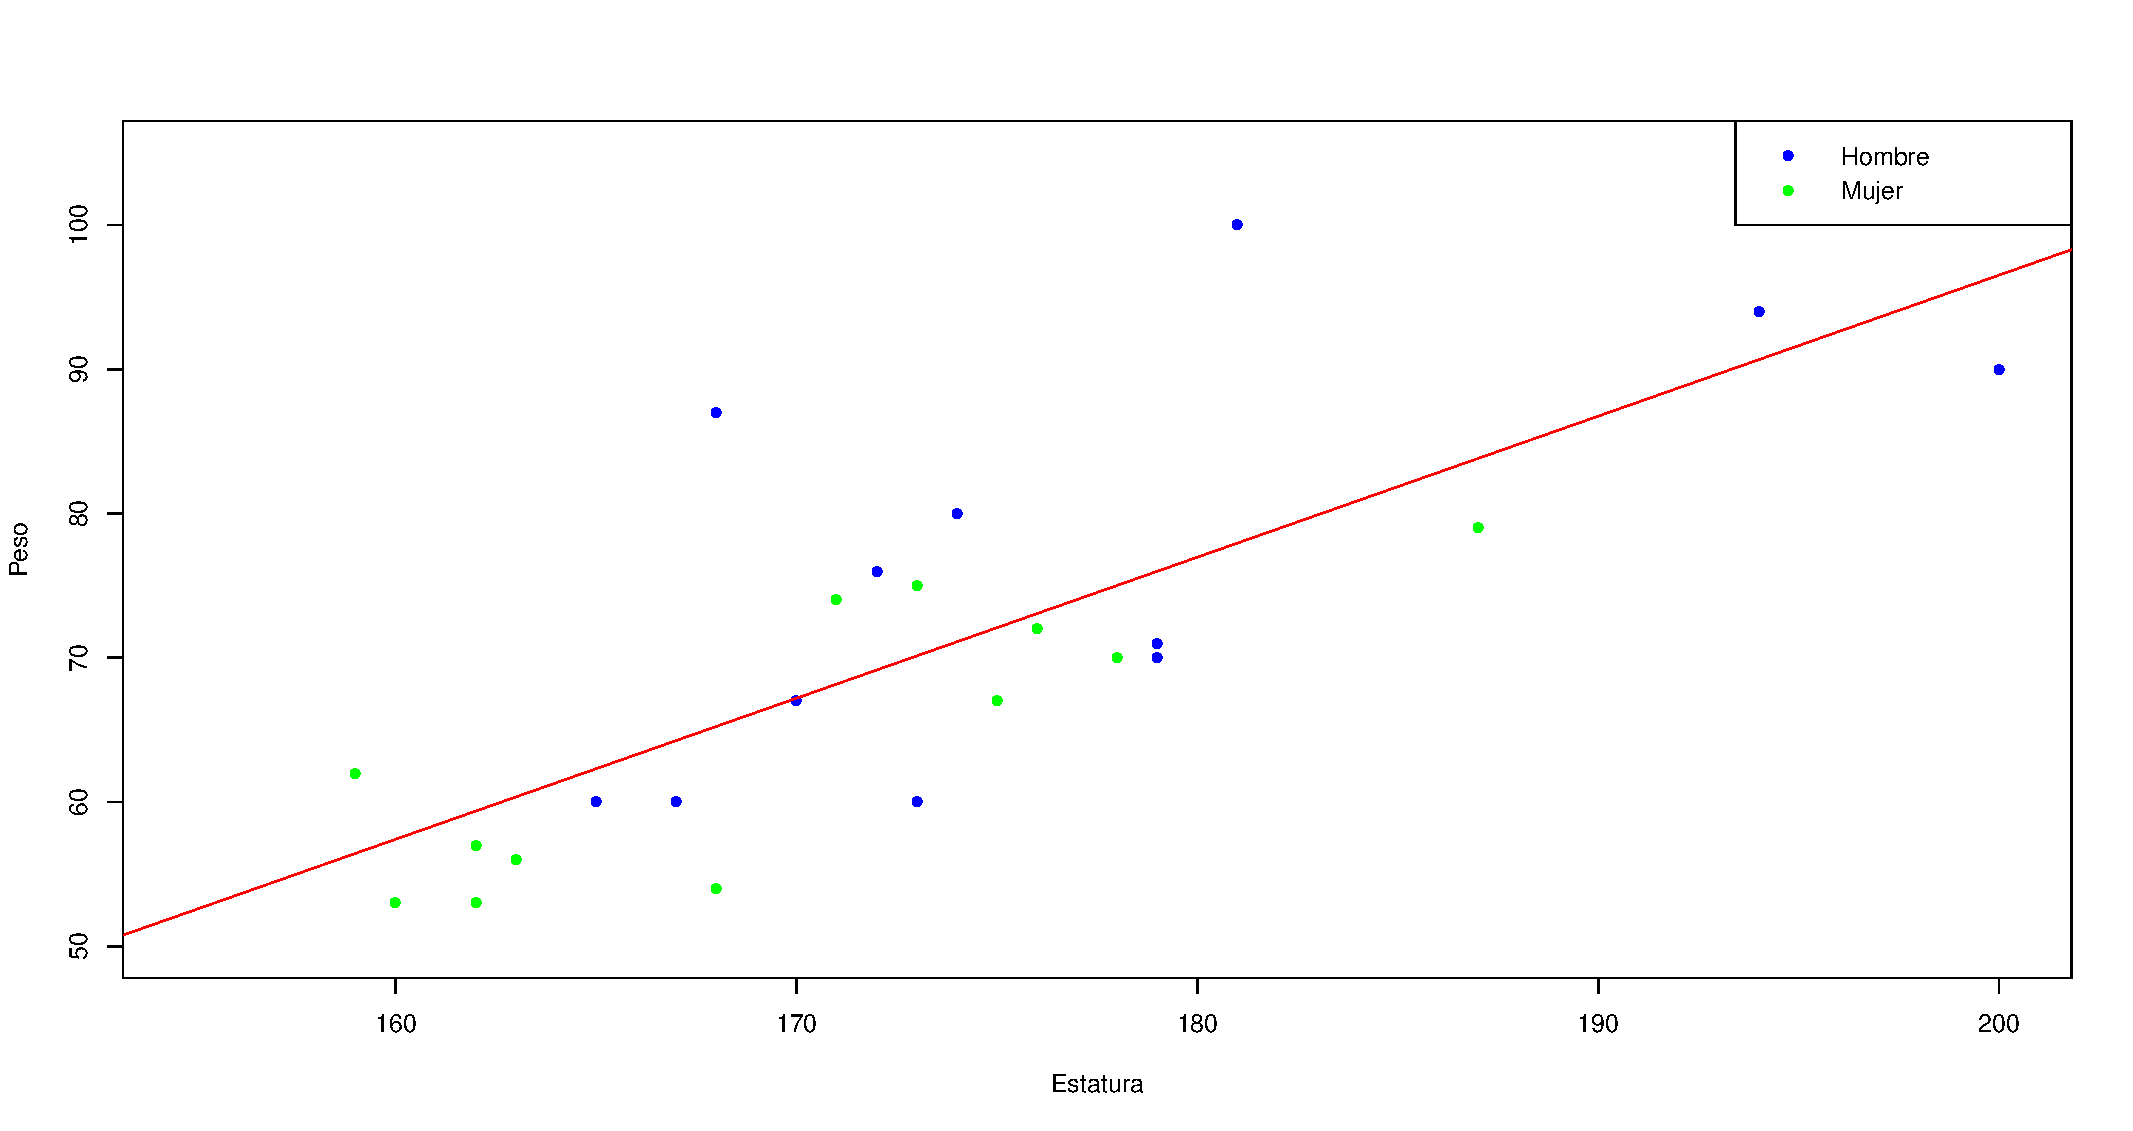
\includegraphics[width=11cm]{imagenes/1.pdf}
        \caption{Gráfica de dispersión con la recta ajustada}
        \label{fig:Densidad}
    \end{center}
\end{figure}
\end{frame}

\begin{frame}
\frametitle{Punto 2: Bondad del modelo e interpretaciones}
\begin{itemize}
\item $R^2=0.5754$: El 57.54\% de la variabilidad total de la variable Y:'Peso' es explicada por la variable X:'Estatura'
\item $\beta_{0}=-99.0330$:Este valor del intercepto es para un mejor ajuste del modelo teniendo en cuenta que no tenemos alturas negativas nos ayuda a ajustar el peso en función de la altura
\item $\beta_{1}=0.9778$: Cuando la variable 'Estatura', aumenta en una unidad (1 centímetro), se espera que el 'Peso' de la persona aumente en 0.9778 kg.
\item p-valor $\beta_{0}=0.00425$:Como mi p-valor es menor que 0.05 rechazo mi hipótesis nula y digo que $\beta_{0}$ si es significante para el modelo 
\item p-valor $\beta_{1}=0.0000174$:Como mi p-valor es menor que 0.05 rechazo mi hipótesis nula y digo que $\beta_{1}$ si es significante para el modelo
\end{itemize}
\end{frame}

\begin{frame}
\frametitle{Punto 3:Intervalos de confianza para $\beta_{0}$ y $\beta_{1}$}
\begin{itemize}
\item $\beta_{0}$: (-163.456 ; -34.610)  ; El verdadero valor de $\beta_{0}$ está entre -163.456 y -34.610 con una confianza del 95\%
\item $\beta_{1}$: (0.6063928 ; 1.3492072) ; El verdadero valor de $\beta_{1}$ está entre 0.6064 y 1.3492 con una confianza del 95\%
\end{itemize}

\end{frame}
\begin{frame}
\frametitle{Punto 4:Inclusión de la variable 'Sexo' al modelo}
~\\ Para incluir la variable sexo al modelo, recodificamos la variable en términos binarios, la cual tomaba el valor 0 cuando es mujer y 1 cuando es hombre,además, es claro que la variable 'Altura', también depende del sexo de la persona (normalmente la media de la estatura de los hombres es mayor a la media de las mujeres), por lo cuál se tuvo en cuenta este cambio en la altura dependiendo del sexo, en pocas palabras, se tuvo en cuenta la interacción entre estas dos variables ('Altura' y 'Sexo'), el modelo ajustado incluyendo la variable 'Sexo' fue el siguiente:
~\\ $$Peso=-92.8094+0.9271 Altura+ 19.4939 Sexo -0.0813(Altura\cdot Sexo)$$
\end{frame}
\begin{frame}
\frametitle{Punto 5:Comparación de modelos}
\begin{table}[!htb]
\caption{Tabla comparativa entre los modelos ajustados}\label{Tabla1}
\begin{center}
\begin{tabular}{ccc}
\hline
 & Peso-Altura & Peso-Altura,Sexo \\ 
\hline
$R^2_{ajustado}$ & 0.5561 & 0.5574 \\ 
 
$CME=\sigma^2$ & 77.33809 & 77.10571 \\ 
\hline 
\end{tabular}
\end{center}
\end{table}
\end{frame}

\begin{frame}
\frametitle{Punto 6:Inclusión de la variable 'Edad' en el modelo}
~\\ El modelo ajustado incluyendo la variable edad, es el siguiente:
~\\ $$Peso=-108.63737+0.91223 Altura+14.77551 Sexo+0.97851 Edad$$
$$-0.05999(Altura\cdot Sexo)$$
\end{frame}

\begin{frame}
\frametitle{Punto 6:Comparación de todos los modelos}
\begin{table}[!htb]
\centering
\caption{Tabla comparativa entre los modelos ajustados}\label{Tabla1}
\resizebox{12cm}{!} {
\begin{tabular}{cccc}
\hline
 &Peso-Altura&Peso-Altura,Sexo&Peso-Altura,Sexo,Edad \\ 
\hline
$R^2_{ajustado}$ &0.5561&0.5574&0.5572 \\ 
 
$CME=\sigma^2$ &77.33809&77.10571&77.14896 \\ 
\hline 
\end{tabular}
}
\end{table}
\end{frame}


\end{document}